\documentclass[tikz]{standalone}
\usepackage{pgfplots}
\pgfplotsset{compat=1.15}
\usepackage{mathrsfs}
\usetikzlibrary{arrows,calc}
\usepackage{tkz-euclide}
\pagestyle{empty}

\definecolor{AngleClr}{rgb}{0,0.39215686274509803,0}
\definecolor{ShapeClr}{rgb}{0.6,0.2,0}

\begin{document}

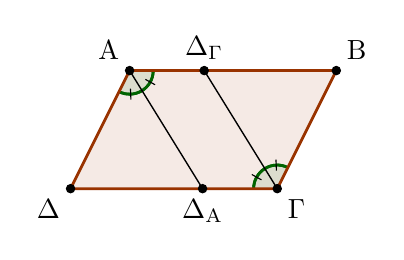
\begin{tikzpicture}[scale=.75]
\tkzSetUpLine[line width=1pt,color=black]
\tkzSetUpPoint[fill=black]

\tkzDefPoints{0/0/D,3.5/0/C,1/2/A,4.5/2/B}

\tkzInterLL(A,C)(B,D) \tkzGetPoint{O}

\tkzDefLine[bisector,normed](B,A,D) \tkzGetPoint{x}
\tkzDefLine[bisector,normed](B,C,D) \tkzGetPoint{y}

\tkzInterLL(A,x)(C,D) \tkzGetPoint{DA}
\tkzInterLL(C,y)(A,B) \tkzGetPoint{DC}

\tkzFillPolygon[fill=ShapeClr,fill opacity=0.1](A,B,C,D)

\tkzFillAngles[fill=AngleClr,size=.4,fill opacity=0.1](D,A,DA DA,A,B B,C,DC DC,C,D)
\tkzMarkAngles[line width=1pt,color=AngleClr,size=.4](D,A,DA DA,A,B B,C,DC DC,C,D)
\tkzMarkAngles[mark=|,mksize=2,line width=1pt,size=.4,color=AngleClr](D,A,DA DA,A,B B,C,DC DC,C,D)

\tkzDrawSegments[line width=0.5pt,color=black](A,DA C,DC)

\tkzDrawPolygon[color=ShapeClr](A,B,C,D)
\tkzDrawPoints[size=3](A,B,C,D,DA,DC)
\tkzLabelPoint[above left](A){$\rm A$}
\tkzLabelPoint[above right](B){$\rm B$}
\tkzLabelPoint[below right](C){$\rm \Gamma$}
\tkzLabelPoint[below left](D){$\rm\Delta$}
\tkzLabelPoint[above](DC){$\rm \Delta_\Gamma$}
\tkzLabelPoint[below](DA){$\rm \Delta_A$}

\end{tikzpicture}
\end{document}
